\section{Designing a profile with one surviving angular mode}
\label{sec:rosen-reference-packet}
\label{sec:radial-models}

The geometric construction asks for a nonradial height which becomes
exactly constant at two ends.  Its first-order version already tells us
what the radial metric must do.  For
\[
 u(r,\theta)=u_0(r)+\sum_{\substack{j\ge2\\j\ {
m even}}}u_j(r)e_j(\theta),
 \qquad e_j(\theta)=\sqrt2\cos(j\theta),
\]
the linearized equation is a family of ordinary differential equations:
\begin{equation}\label{eq:rad-eq-modal-operator}
 L_ju=(wu')'-j^2\frac{w'}r u,
 \qquad
 \mathscr L_wu=(wu_r)_r+\frac{w'}r u_{\theta\theta}.
\end{equation}
We want exactly one endpoint-flat solution among the nonzero angular
modes.  We choose its frequency to be two, the first frequency compatible
with the half-turn symmetry used in the geometric closure.  The
nonlinear equation will create the higher even frequencies, so they
must all have inverses on this same profile.

There are two freedoms here.  The shape of a local profile determines
its oscillation and its spectrum.  Multiplying that profile by a positive
constant changes its flux scale without changing its homogeneous
solutions.  We use the first freedom to obtain explicit local models,
and the second to prevent a resonance when neighboring models are
joined.  This separation is the organizing idea of the construction.

\subsection{What the radial construction must supply}

We record the analytic interface before choosing the models.  The estimates
are stated in the original radius, so no change of source measure is
implicit.  Angular brackets denote normalized angular average.

\begin{definition}[The three endpoint scales]\label{def:radial-weights}
The cells approaching either endpoint are indexed by $n\ge N$.  Set
\begin{equation}\label{eq:rad-eq-endpoint-weights}
 A_n\asymp e^{-n^2},\qquad
 S_n=\frac23 n^3,\quad H_n=e^{-S_n},\qquad
 q_n=n^{5/2}\log(e+n),\quad \mathcal E_n=e^{q_n}.
\end{equation}
A coefficient estimate of order $s$ on cell $n$ means an estimate by
$C_s\mathcal E_n^{C_s}$.  The same notation on the finitely many central
pieces denotes fixed positive constants.  A cell includes fixed portions
of its neighboring positive intervals; a bounded enlargement changes
its index by at most a fixed integer.
\end{definition}

The length scale $A_n$ measures how much room is available.  The much
smaller quantity $H_n$ will measure the decay of the distinguished
solution.  The intermediate weight $\mathcal E_n$ pays for taking
reciprocals and derivatives of the coefficients.  Section~\ref{sec:radial-tails}
derives all three scales from a continuous construction; they are not
independent hypotheses about an unknown profile.

Choose a smooth partition $\vartheta_m$ with bounded overlap on the
cells and the finite middle; $m$ records both the endpoint and the cell
index.  For fixed $0<\gamma<1$, write
\begin{equation}\label{eq:rad-eq-source-norm}
 \|(f,c)\|_{Y_{\gamma,s}}^2
 =|c|^2+\sum_m\mathcal E_m^{2M_0}H_m^{-2\gamma}
       \|\vartheta_m f\|_{L^2(dr)H^s(\T)}^2.
\end{equation}
The output norm at angular order zero replaces
$\mathcal E_m^{2M_0}$ by $\mathcal E_m^{-2M_1}$.
In that norm the zero mode is written $a_L\chi_L+v_0$, where
$\chi_L$ is a fixed smooth function equal to one near the left endpoint
and zero near the right.  We include $|a_L|$ and the scalar unknown
below in the output norm.

\begin{proposition}[The fixed radial reference]\label{prop:rad-fixed-theorem}
There is a positive smooth profile $w_*$ on a finite interval
$(r_-,r_+)$, flat at both endpoints, with only simple interior zeros of
$w_*'$.  It has the following properties.

There is a nonzero endpoint-flat function $\phi_*$ with
$L_2\phi_*=0$.  This is the whole endpoint-flat kernel at frequency two;
the kernel is zero at every even frequency $j\ge4$.  Every component
of $\{w_*'<0\}$ has travel angle $T_m$ satisfying
\begin{equation}\label{eq:rad-eq-optical-margin}
 |\sin(kT_m)|\ge\gamma_m/|k|\quad(k\ge1),
 \qquad \gamma_m^{-1}\le\mathcal E_m^{C},
 \qquad T_m/\pi\text{ is quadratic irrational}.
\end{equation}
There is a smooth $\chi_*$ supported in a positive component such that
\begin{equation}\label{eq:rad-eq-target-border}
 g_*=L'_{2,w_*}[w_*\chi_*]\phi_*,\qquad
 \int g_*\phi_*\,dr=1,\qquad
 \ell_*u=\int g_*u_2\,dr.
\end{equation}
The bordered operator
\begin{equation}\label{eq:rad-eq-bordered-reference}
 \mathbb L_{w_*}(u,\nu)
   =\bigl(\mathscr L_{w_*}u+\nu g_*e_2,\ell_*u\bigr)
\end{equation}
has a two-sided inverse on compatible sources,
$\int\langle f\rangle\,dr=0$, with right endpoint height zero and
one free left endpoint constant.  For every compact interval
$[\gamma_-,\gamma_+]\Subset(0,1)$ there are fixed $M_0,M_1$ for which
this inverse is bounded from $Y_{\gamma,0}$ to the output norm above,
uniformly for $\gamma$ in that interval.  One radial derivative costs
at most one additional angular derivative of the source.  The profile,
its kernel and the border are the same for all these exponents.
\end{proposition}

Here $L'_{2,w}[v]\phi=(v\phi')'-4v'\phi/r$ is the derivative
with respect to the radial profile; the source is still a density in $dr$.
The proof occupies this section and the next two.  Its conclusion is a
base inverse estimate, including the endpoint realization.  Higher total
orders will be recovered from the differential equation after the
weighted spaces have been introduced.  Keeping these two tasks separate
avoids making the choice of geometry depend on the eventual regularity
order.

\subsection{Turning a spectral potential into a radial metric}

It is easier to design the spectrum before designing the radius.  Let
$X$ be a model coordinate, let $r_X=v>0$, and choose a positive density
$\mathcal P$.  Put
\begin{equation}\label{eq:rad-eq-sc0}
 \begin{gathered}
 w(r(X))=\lambda\mathcal P(X)v(X),\qquad
 \rho=-\frac{r_{XX}+(\mathcal P_X/\mathcal P)r_X}{r},\qquad
 V_0=\frac{(\sqrt{\mathcal P})_{XX}}{\sqrt{\mathcal P}},\\
 L_j(\mathcal P^{-1/2}\psi)
   =-\frac{\lambda\sqrt{\mathcal P}}{v}
      \bigl(-\psi_{XX}+(V_0-j^2\rho)\psi\bigr).
 \end{gathered}
\end{equation}
Indeed $wu_r=\lambda\mathcal P u_X$, and differentiating this expression
and using the definition of $\rho$ gives the identity.  Thus a
Schr\"odinger model determines the radial equation once its radius
satisfies the displayed linear equation and remains increasing.
The factor $\lambda$ is absent from the homogeneous model.

Our two choices have complementary jobs.  The central oscillator
retains the desired zero mode.  The Morse models near the ends have
explicit nonzero gaps, but are short enough in radius to accumulate
at a finite point.  Figure~\ref{fig:two-spectral-models} illustrates the
potentials; it is their solvable spectra, rather than the qualitative
shapes alone, that make them useful.

\begin{figure}[htbp]
\centering
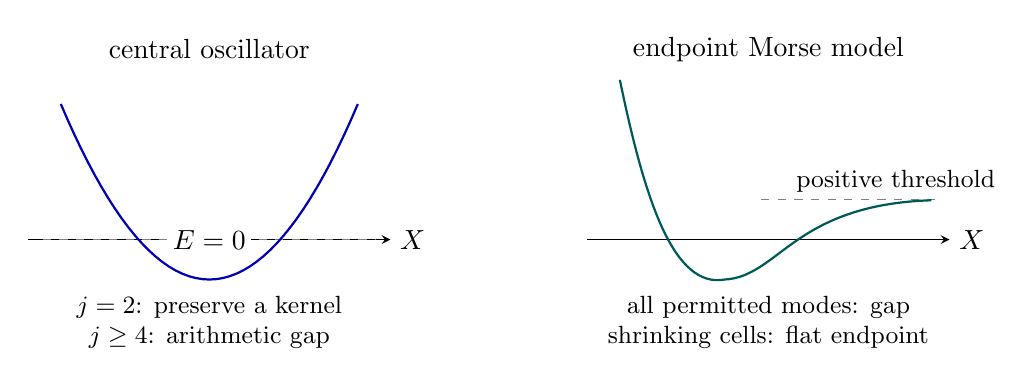
\begin{tikzpicture}[x=.92cm,y=.78cm,>=stealth]
\begin{scope}
\draw[->] (-2.5,0)--(2.5,0) node[right] {$X$};
\draw[dashed,gray] (-2.3,0)--(2.3,0);
\draw[thick,blue!70!black,domain=-2.05:2.05,samples=45]
 plot (\x,{.68*\x*\x-.65});
\node[align=center] at (0,3.1) {central oscillator};
\node[fill=white,inner sep=2pt] at (0,0) {$E=0$};
\node[align=center,font=\small] at (0,-1.35)
 {$j=2$: preserve a kernel\\$j\ge4$: arithmetic gap};
\end{scope}
\begin{scope}[xshift=7.1cm]
\draw[->] (-2.5,0)--(2.5,0) node[right] {$X$};
\draw[dashed,gray] (-.1,.65)--(2.3,.65);
\draw[thick,teal!70!black]
 (-2.05,2.6) .. controls (-1.7,.6) and (-1.3,-.8) .. (-.6,-.65)
 .. controls (.15,-.6) and (.35,.57) .. (2.25,.64);
\node[align=center] at (0,3.1) {endpoint Morse model};
\node[anchor=west,font=\small] at (.25,.95) {positive threshold};
\node[align=center,font=\small] at (0,-1.35)
 {all permitted modes: gap\\shrinking cells: flat endpoint};
\end{scope}
\end{tikzpicture}
\caption{The two full-line spectral models, drawn schematically with an
arbitrary vertical scale.  Only finite pieces are used in the surface.
Positive end regions separate those pieces when they are joined.}
\label{fig:two-spectral-models}
\end{figure}

\subsection{The central oscillator}
\label{subsec:rad-central-singlepoint}

Set
\begin{equation}\label{eq:rad-eq-sc1}
 A_c=1/\sqrt2,\qquad a_c=\sqrt{4A_c-2},\qquad
 c_c=3A_c-2>0,\qquad \alpha_c=(c_c+1)/2.
\end{equation}
Take $\mathcal P=e^{-2a_cX}$ and $\rho=A_c-X^2$.
Then the model operator is
\[
 H_{j,c}=-\partial_X^2+j^2X^2+a_c^2-j^2A_c.
\]
Its standard oscillator spectrum is
\begin{equation}\label{eq:central-spectrum-new}
 E_{m,j}=j(2m+1)+a_c^2-j^2A_c,\qquad m=0,1,\ldots;
\end{equation}
see \cite[\S8.3, equations (8.33)--(8.42)]{Teschl2009}.
The choice of $a_c$ sets $E_{0,2}=0$.  The irrational choice of $A_c$
keeps the other even frequencies away from zero.

Here is the quantitative part of that last assertion.  Put
$\Phi_j=jA_c-a_c^2/j$.  For even $j\ge4$,
\[
 N_j:=j^2/2-\Phi_j^2=2A_ca_c^2-a_c^4/j^2
\]
lies between $13/4-3\sqrt2/2$ and $4-2\sqrt2$, so its distance
from the integers is at least
$\delta=\tfrac34(3-2\sqrt2)>0$.
If $|E_{m,j}|<1$, then $2m+1=\Phi_j+E_{m,j}/j$ and
$2m+1+\Phi_j<2j$.  Since $j^2/2-(2m+1)^2$ is an integer,
\[
 \delta\le |(2m+1)^2-\Phi_j^2|<2|E_{m,j}|.
\]
This also yields the bound when $|E_{m,j}|\ge1$.  At $j=2$ the levels
are $4m$.  Consequently
\begin{equation}\label{eq:rad-eq-sc3}
 \|H_{j,c}^{-1}\|\le2/\delta\quad(j\ge4\text{ even}),
 \qquad \ker H_{2,c}=\operatorname{span}\{e^{-X^2}\},
\end{equation}
and the reduced inverse at $j=2$ has norm $1/4$.
We use the closed quadratic-form realization in these statements.

We still need an increasing radius; an arbitrary solution of the radius
equation would not suffice.  An explicit positive one is
\begin{equation}\label{eq:rad-eq-sc6}
 \psi_1(X)=e^{-X^2/2}\int_0^\infty
 t^{\alpha_c-1}e^{-t^2/2+\sqrt2Xt}\,dt,
 \qquad r=e^{a_cX}\psi_1,\qquad \upsilon=r_X/r.
\end{equation}
An integration by parts in $t$ shows that
$\psi_1''=(X^2+c_c)\psi_1$.
The function is positive, while $\psi_1,\psi_1'$ tend to zero as
$X\to-\infty$.  Hence $\psi_1''>0$ implies $\psi_1'>0$ and
$\upsilon=a_c+\psi_1'/\psi_1>a_c$.  Using
$c_c-a_c^2+A_c=0$ gives
$r_{XX}-2a_cr_X+(A_c-X^2)r=0$, exactly the equation in
\eqref{eq:rad-eq-sc0}.  In particular this spectral model really is a
radial metric.

For later cuts, the needed end estimates are
\begin{equation}\label{eq:rad-eq-sc6a}
 \upsilon=
 \begin{cases}
 -X+a_c-\alpha_c/X+O(X^{-3}),&X\to-\infty,\\
 X+a_c+(\alpha_c-1)/X+O(X^{-3}),&X\to+\infty.
 \end{cases}
\end{equation}
These estimates hold after any fixed number of derivatives.  For
$X=-L$, substitute $t=z/(\sqrt2L)$ in the integral; the remaining
integral is $\Gamma(\alpha_c)(1+O(L^{-2}))$ and can be differentiated
under its exponentially integrable majorant.  For $X>0$, complete the
square and expand $t^{\alpha_c-1}$ about $\sqrt2X$ against the Gaussian;
the part $|t-\sqrt2X|>X/2$ is exponentially small.  Logarithmic
differentiation gives \eqref{eq:rad-eq-sc6a}.
Thus $r$ ranges from zero to infinity, and
$\upsilon\asymp1+|X|$.

The surviving radial height and its logarithmic slope are
\begin{equation}\label{eq:rad-eq-sc2}
 \phi_0=e^{a_cX-X^2},\qquad
 \frac{\partial_y\phi_0}{\phi_0}=\frac{a_c-2X}{\upsilon}
       \longrightarrow 2\ \text{on the left},\quad -2\ \text{on the right},
 \qquad y=\log r.
\end{equation}
Writing $w=re^f$, the radius equation also gives
\begin{equation}\label{eq:rad-eq-sc6b}
 1+f_y=\frac{X^2-A_c}{\upsilon^2}\longrightarrow1.
\end{equation}
We may therefore cut far enough out that both end regions are positive
and have uniformly bounded logarithmic-coordinate jets.  There are
just two simple turning points in the retained middle.  Its travel angle
is $\pi A_c/2=\pi/(2\sqrt2)$, whose sine divisors satisfy
$|\sin(kT)|\ge c/k$ by the integer norm $|k^2-8m^2|\ge1$.

There is one measure conversion worth settling now.  Define
\begin{equation}\label{eq:rad-eq-ha2}
 \varpi=12w/r^2,\quad B_j=-\varpi^{-1}L_j,
 \qquad
 \|u\|_{L^2(\varpi dr)}^2=12\lambda\|\upsilon\psi\|_2^2,
 \quad u=\mathcal P^{-1/2}\psi.
\end{equation}
The inverse in this measure contains
$\upsilon H_{j,c}^{-1}\upsilon$, not merely $H_{j,c}^{-1}$.
It is uniformly bounded.  Indeed
$V_j\ge c j^2\upsilon^2-Cj^2$ and the spectral gap first give
$\|\upsilon H_{j,c}^{-1}\|\le C$; taking adjoints gives the bound
on the other side.  For $\psi=H_{j,c}^{-1}(\upsilon F)$,
\[
 cj^2\|\upsilon\psi\|_2^2
 \le \|\upsilon\psi\|_2\|F\|_2+Cj^2\|F\|_2^2,
\]
and absorption yields the two-sided weight bound.  At $j=2$, add the
projection onto $e^{-X^2}$, apply the same argument, and subtract that
projection.  Its weighted norm is finite.

We will temporarily border mode two by a compact function $g_0$ with
$\int g_0\phi_0\,dr=1$ and row $\ell_0u=\int g_0u\,dr$.
The source obstruction is removed by pairing with $\phi_0$; adding a
multiple of $\phi_0$ fixes the row.  Thus this bordered inverse has the
same bounds.  Normalize its Hilbert scalar so that under a height
rescaling $w\mapsto\lambda w$ one has
$g_0\mapsto\sqrt\lambda g_0$, $\phi_0\mapsto\phi_0/\sqrt\lambda$.
Both the row and column then have bounded Hilbert norm.  This is an
auxiliary border, changed to \eqref{eq:rad-eq-target-border} after all
geometric choices have been made.

\subsection{Morse models: two quantitative gaps from one irrationality}

For the tails take $\mathcal P=1$ and
\[
 \rho(X)=A(e^{-X}-e^{-2X})-B,
 \qquad H_{j,M}=-\partial_X^2-j^2\rho,
 \qquad A>4B>0.
\]
The essential spectrum starts at $j^2B$; below it the simple eigenvalues
are
\begin{equation}\label{eq:rad-eq-fs1}
 E_{m,j}=j^2B-(\alpha_j-m)^2,
 \qquad \alpha_j=(j\sqrt A-1)/2,\qquad 0\le m<\alpha_j.
\end{equation}
This is the Morse spectrum \cite{Morse1929}.  For completeness, the
factorization which fixes its normalization is short.  With
$\omega=j\sqrt A$ and $D_\alpha=\partial_X+\alpha-\omega e^{-X}$,
\[
 H_\alpha=D_\alpha^*D_\alpha+j^2B-\alpha^2,
 \qquad
 H_{\alpha-1}=D_\alpha D_\alpha^*+j^2B-\alpha^2.
\]
The null function of $D_\alpha$ is
$e^{-\alpha X-\omega e^{-X}}$, square integrable exactly for
$\alpha>0$.  Descending by integers removes one ground state at a
time.  At $-1<\alpha\le0$,
$H_\alpha-j^2B=D_0^*D_0-2\omega\alpha e^{-X}\ge0$;
there are no further levels.  Reversing the intertwining recovers every
level in \eqref{eq:rad-eq-fs1}.  The quadratic-form realization justifies
these identities by cutoff integration.  At the left end the potential
is confining, and at the right it approaches $j^2B$ exponentially;
the usual compact-perturbation argument gives the stated essential
threshold \cite[Theorem~6.19]{Teschl2009}.  These facts suffice for the
resolvent estimates below, all at energy zero.

Choose a nonsquare integer $d$ and set
\begin{equation}\label{eq:rad-eq-rm5}
 A=(d^{-1/2}+2d^{-9/2})^2,
 \qquad B=d^{-9}.
\end{equation}
For positive integers $j$ and odd $M$,
\[
 |j/\sqrt d-M|\ge (4j\sqrt d)^{-1}.
\]
If the difference is smaller than $1/2$, this follows by factoring the
nonzero integer $j^2-dM^2$; otherwise it is immediate.  At a discrete
level write $\kappa=(j\sqrt A-M)/2>0$.  Since
$\sqrt A-2\sqrt B=d^{-1/2}$,
\[
 |j^2B-\kappa^2|
 \ge \frac{j\sqrt B}{2}|j/\sqrt d-M|
 \ge\frac1{8d^5}.
\]
Together with the threshold $j^2d^{-9}$ this proves
\begin{equation}\label{eq:rad-eq-rm1}
 \|H_{j,M}^{-1}\|\le8d^9\qquad(j\ge2).
\end{equation}

The same irrationality controls the characteristic return.  The change
$t=e^{-X}$ gives
\begin{equation}\label{eq:rad-eq-rm2}
 T=\int_{\rho>0}\sqrt\rho\,dX
   =\pi(\sqrt A/2-\sqrt B)=\frac\pi{2\sqrt d}.
\end{equation}
To evaluate the integral, write the positive quadratic as
$A(t-t_-)(t_+-t)$ and use $t=c+h\cos\xi$; the elementary integral is
$\pi(c-\sqrt{c^2-h^2})$.  Here $t_-+t_+=1$ and
$t_-t_+=B/A$.  Factoring the integer $k^2-4dm^2$, with $m$ the nearest
integer to $k/(2\sqrt d)$, yields
\begin{equation}\label{eq:rad-eq-morse-small-divisor}
 |\sin(kT)|\ge(3k\sqrt d)^{-1}\qquad(k\ge1).
\end{equation}
For $k<\sqrt d$ use $m=0$ directly; otherwise the factorization gives
distance at least $(6k\sqrt d)^{-1}$ from the integers.
Thus one parameter choice supplies both local spectral separation and
return-angle separation.  They remain distinct conditions when the
models are joined: a junction can create a new spectral resonance
without changing any individual travel angle.  The next section deals
with that remaining freedom.
